\section{Simulation study}
\label{sim}

We apply the hierarchical model to simulations from a max-autoregressive process. For $i=1,\ldots,R$, choose $\theta_i\in(0,1]$. Let $W_{i,1}\ldots,W_{i,n}$ be independent unit Fr{\'e}chet random variables, and define
\begin{align}
Y_{i,1} &= W_{i,1}/\theta_i \nonumber \\
Y_{i,j} &= \max\{(1-\theta_i)Y_{i,j-1}, W_{i,j}\}~~~~~j=2,\ldots,n \label{max}
\end{align}
then $Y_{i,\cdot}$ is stochastic process having extremal index $\theta_i$. We let $R=10$, $n=1000$, and $\theta_1=\cdots=\theta_R$. This construction is intended to somewhat mimic our situation with the climate model.

A single threshold is chosen based off a quantile of all simulations taken together. That is, if we wish to choose as a threshold the $0.95$ quantile, then $u$ is the solution to
\[ 0.95 = \sum_{i=1}^R\sum_{j=1}^n\ind(Y_{i,j} \leq u) \]
It is certainly possible to select a threshold $u_i$ for each sequence. While this is expected to yield better estimates for $\theta_i$, it is not immediately clear how to apply model (\ref{gpmod}) in the hierarchical setting with different thresholds. What threshold should be used when calculating return levels for the population distribution? Or a new replicate $Y^*$? This, of course, leads to the broader question: If one threshold is to be used, how should it be chosen in the hierarchical setting?

Comparisons between models (\ref{ferro}) and (\ref{suveges}) are made using coverage and mean RMSE. With model (\ref{suveges}) we perform the analysis for $K=1,5$.

Let $\theta_0$ denote the true extremal index. $R$ sequences of size $n$ are simulated according to (\ref{max}). The hierarchical model described in section \ref{model} is fit. Posterior samples of $\theta$, denoted $\theta^{(1)},\ldots,\theta^{(M)}$, are obtained via MCMC. From these samples we calculate the 95\% h.p.d. interval and RMSE,
\[ \sqrt{1/M \sum_{k=1}^M\left(\theta^{(k)}-\theta_0\right)^2}. \]
This processes is repeated $B=500$. Coverage is computed by finding the number of intervals containing the true value $\theta_0$ and dividing by $B$. The mean RMSE is calculated as the mean of the RMSE's from the $B$ sets of samples.


Results are shown in Figure \ref{figsim}. Likelihood (\ref{ferro}) produces coverage at or near $1$, which decreases toward the nominal $0.95$ as threshold increases. The RMSE, on the other hand, is increasing with threshold. The pattern holds for the three $\theta_0$'s considered. These results are in agreement with those shown by \cite{ferro2003inference}, Figure 2.

In contrast, model (\ref{suveges}) with $K=1$ has coverage increasing with threshold toward $0.95$. The RMSE is also increasing, but is greater than the RMSE for (\ref{ferro}), except for $\theta_0=0.5$. For $\theta_0=0.9$, the RMSE does drop below that of (\ref{ferro}) at high thresholds. (Waiting for more code to run, to include $K=5$).


\begin{figure}[H]
\begin{center}
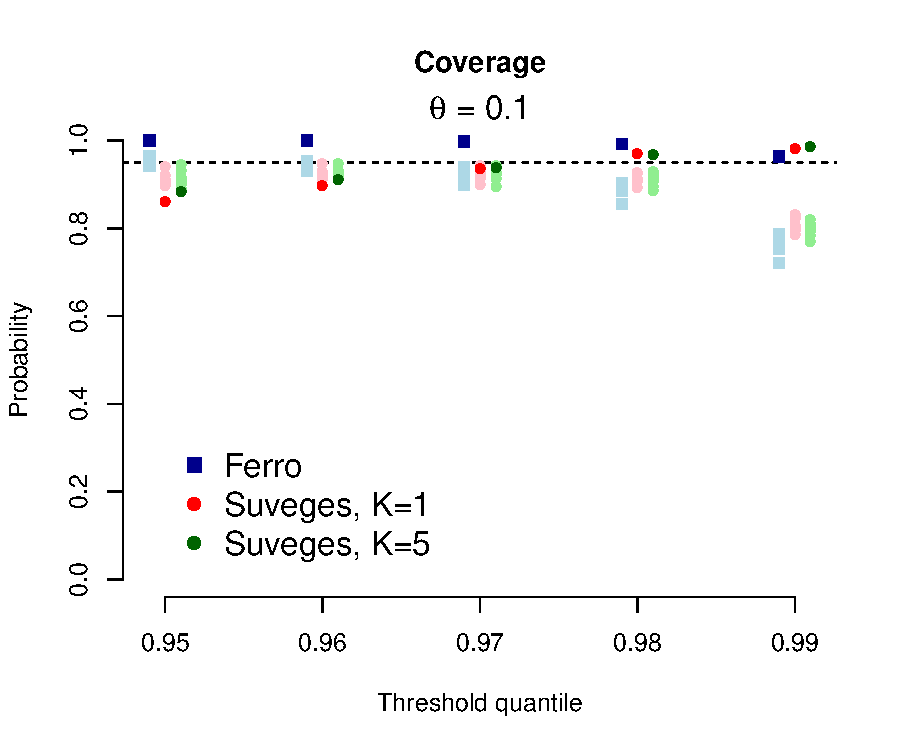
\includegraphics[scale=0.48]{../extremal_comparison/figs/sim_coverage_10.pdf}
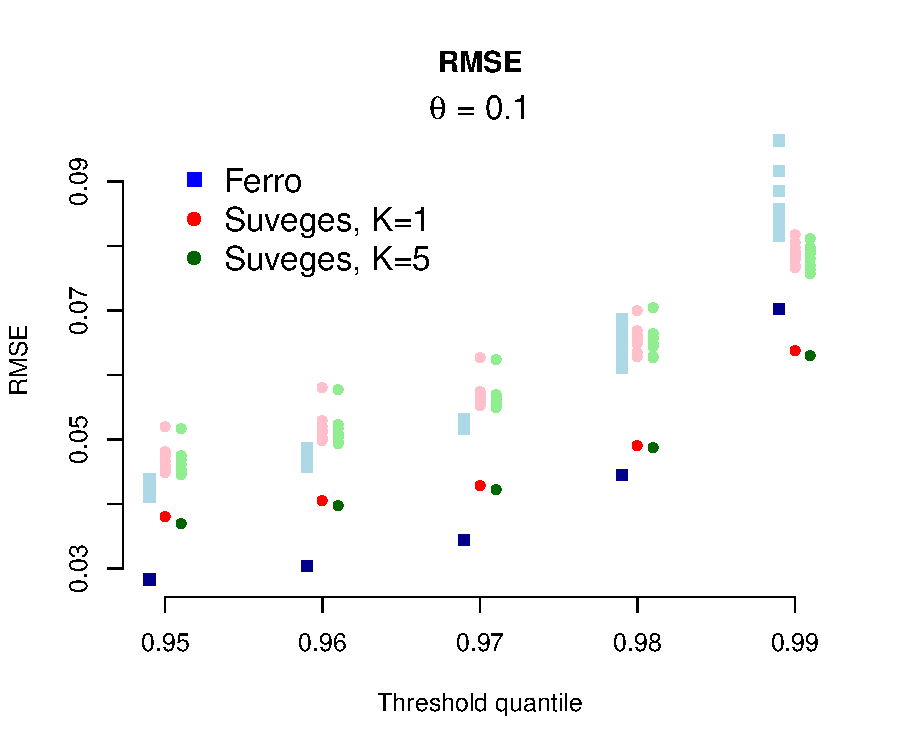
\includegraphics[scale=0.48]{../extremal_comparison/figs/sim_rmse_10.pdf}
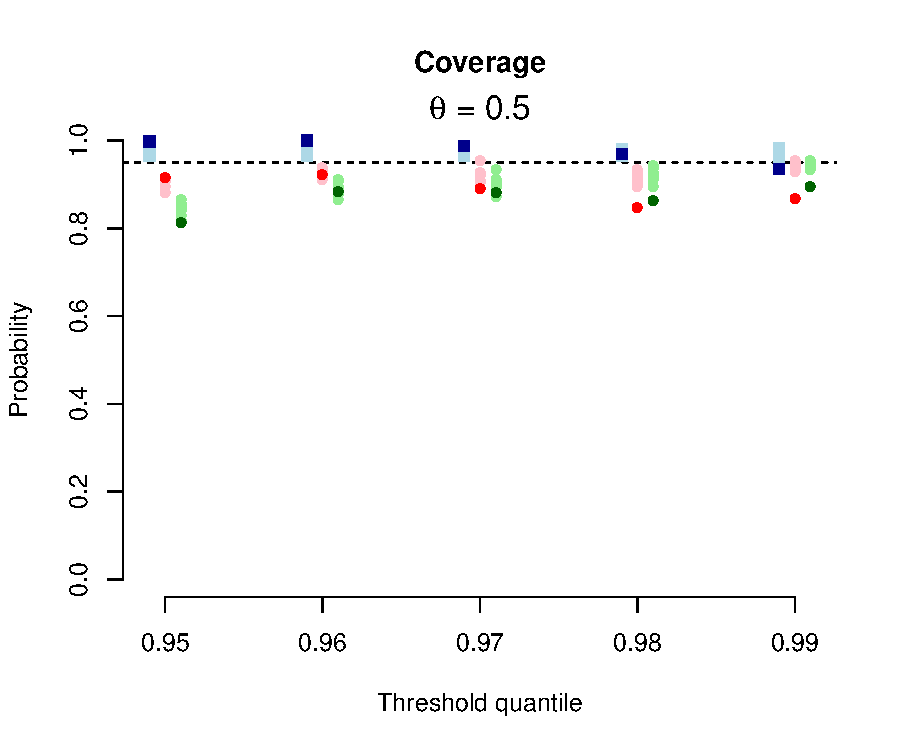
\includegraphics[scale=0.48]{../extremal_comparison/figs/sim_coverage_50.pdf}
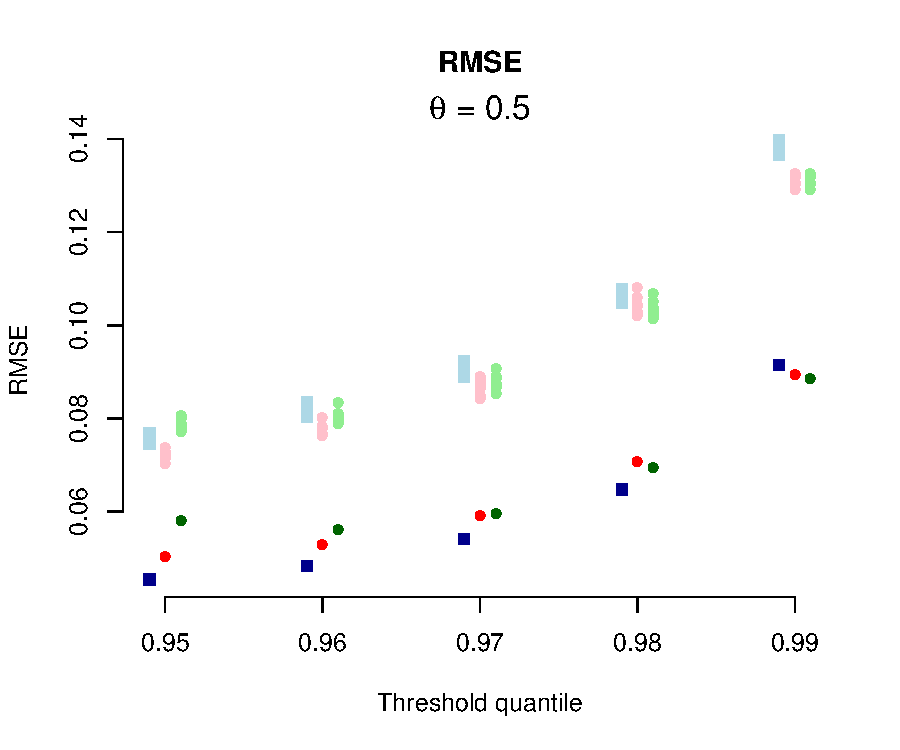
\includegraphics[scale=0.48]{../extremal_comparison/figs/sim_rmse_50.pdf}
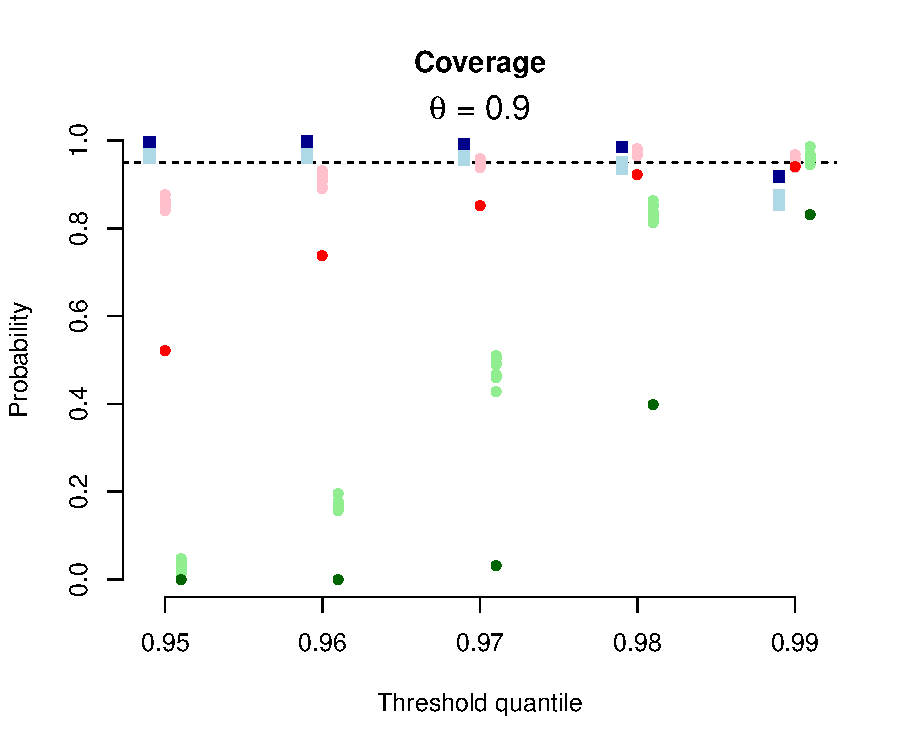
\includegraphics[scale=0.48]{../extremal_comparison/figs/sim_coverage_90.pdf}
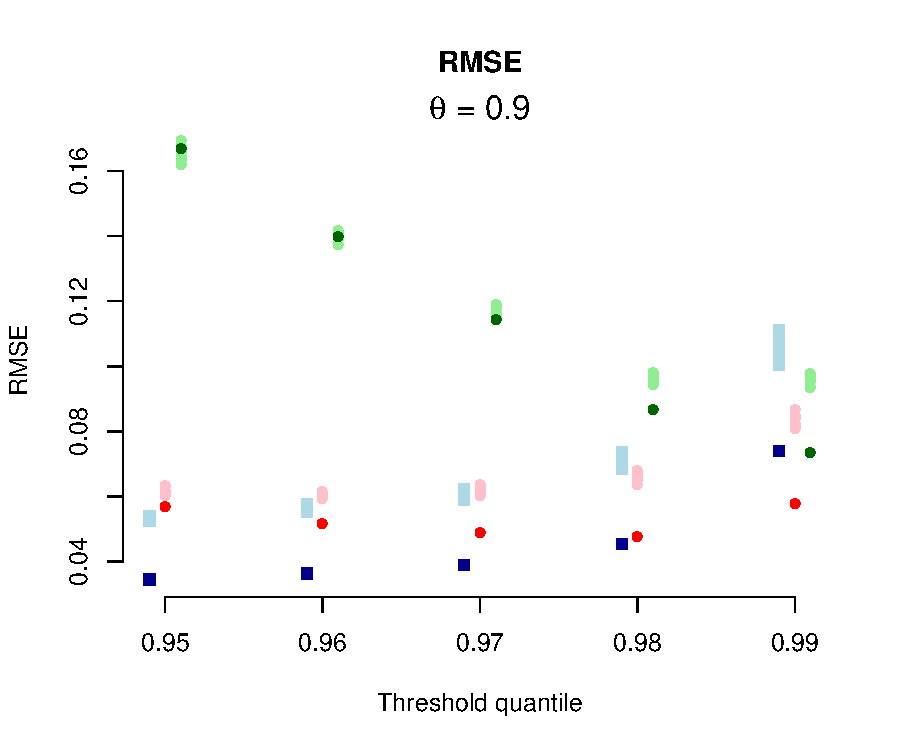
\includegraphics[scale=0.48]{../extremal_comparison/figs/sim_rmse_90.pdf}
\end{center}
\caption{Coverage (left column) and mean RMSE (right) for the two likelihoods in the simulation study. Each row is based on a different extremal index, either $0.10$, $0.50$, or $0.90$. The darker points represent the hierarchical mean ($\theta$), the lighter points are from the individual sequences ($\theta_i$). The nominal coverage probability (0.95) is marked by the dashed horizontal line.}
\label{figsim}
\end{figure}
